\pagebreak
\subsection{Task 3: Building the Client PC and Setting up AD Users}
\subsubsection{Set up a Windows 10 Enterprise client}
\begin{enumerate}[series=task3methodology1]
  \item Download Windows 10 Enterprise from Microsoft Imagine.
  \item Create a new VM in VMware Workstation for the client. Note that this VM is created in VMware Workstation, at the same level as the ESXi VM, and not in the ESXi itself. When creating the VM, ensure that a NAT adapter is included so that the client will be able to see the servers inside ESXi.
  \item Install Windows 10 Enterprise in the VM. Notable steps for this process are as follows:
    \begin{enumerate}[label=(\alph*)]
      \item Create a `Client' account for the machine so that we can login in order to make the changes that are necessary to allow the client to be connected to the domain.
        \begin{figure}[H]
          \centering
          \captionsetup{skip=2pt}
          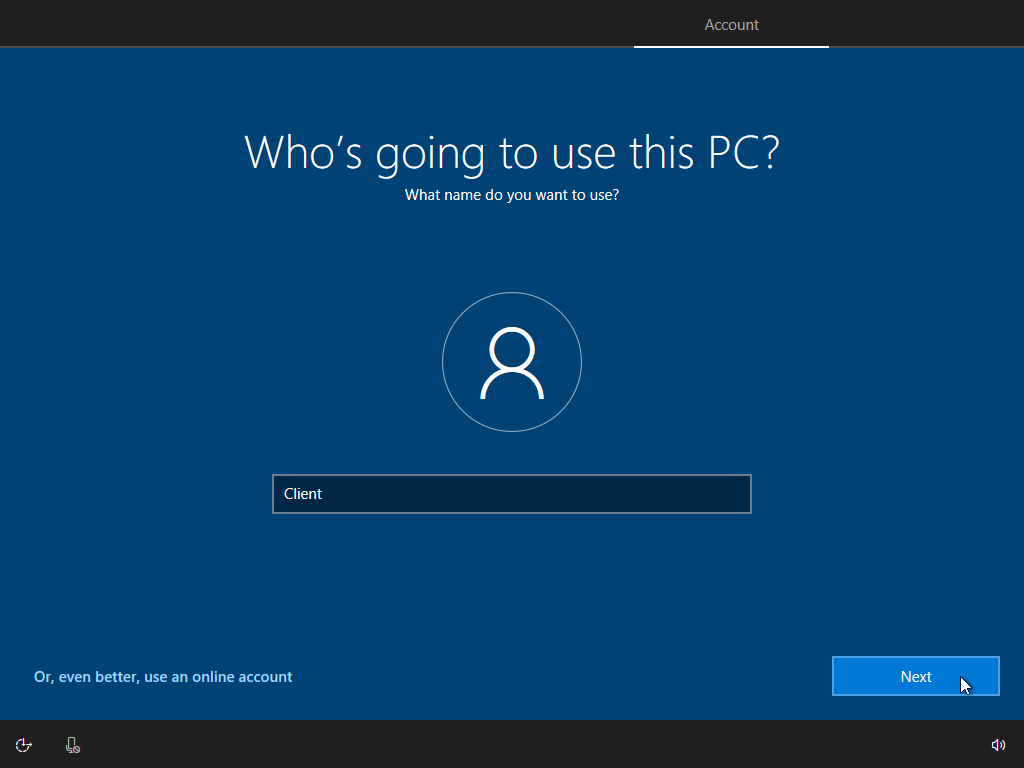
\includegraphics[width=\textwidth]{IY1D403_Windows_10_x64_Client-2018-05-11-20-33-34}
          \caption{Creating a new account during the Windows 10 Client install}
          \label{fig:task3:win10client_01}
        \end{figure}
      \item Select `Don't use'/`No'/`Basic' for the following steps as we are not interested in any of these features for this installation. I thought that selecting the `Enterprise' edition would skip these steps but unfortunately it does not.
        \begin{figure}[H]
          \centering
          \captionsetup{skip=2pt}
          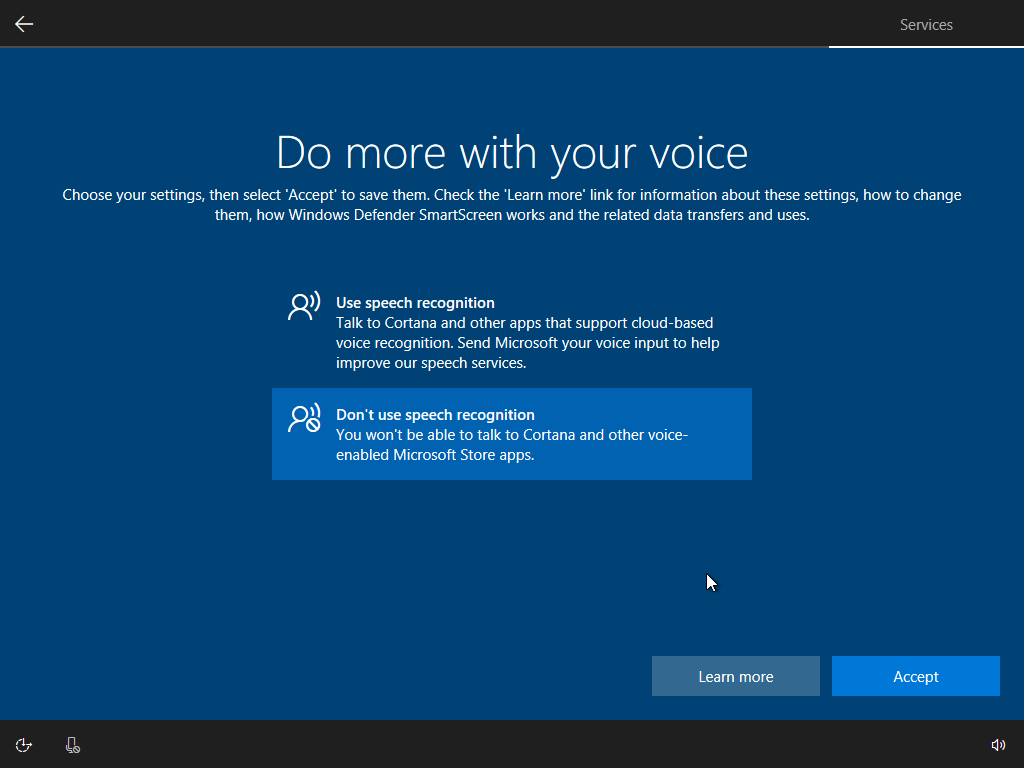
\includegraphics[width=\textwidth]{IY1D403_Windows_10_x64_Client-2018-05-11-20-36-12}
          \caption{Decline to use these extraneous features in the client}
          \label{fig:task3:win10client_02}
        \end{figure}
      \item After completing the installation and logging into the client, set the `Preferred DNS server` to point to the static IP of the Domain Controller.
        \begin{figure}[H]
          \centering
          \captionsetup{skip=2pt}
          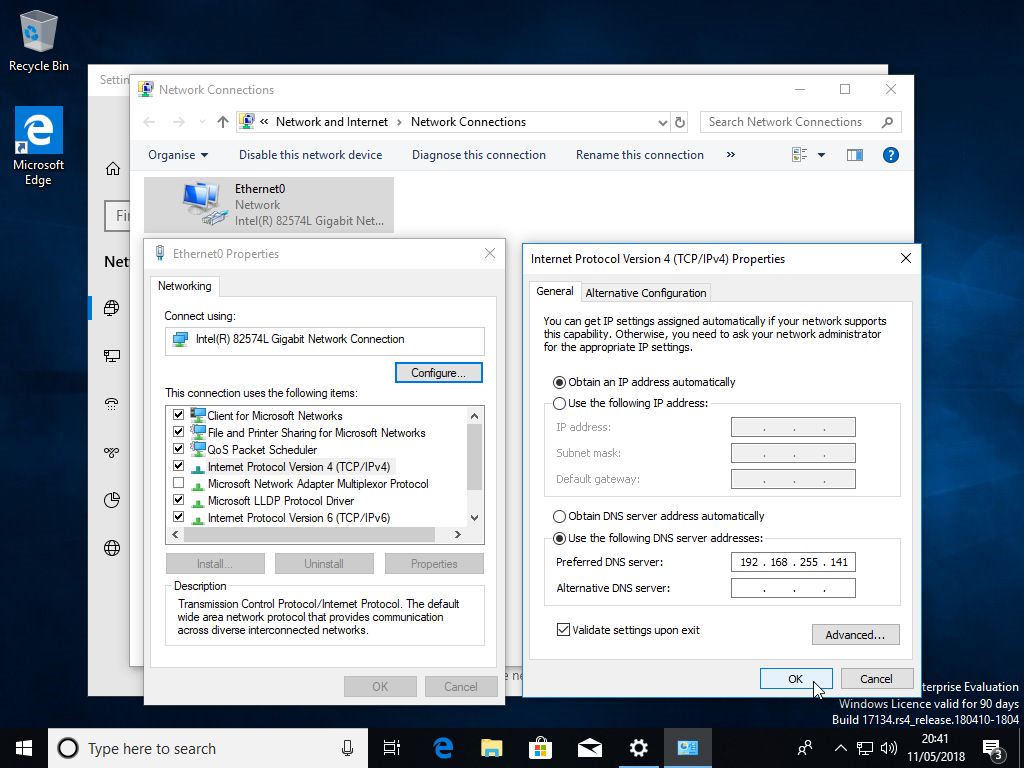
\includegraphics[width=\textwidth]{IY1D403_Windows_10_x64_Client-2018-05-11-20-45-19}
          \caption{Setting the DNS for the client to point to the Domain Controller}
          \label{fig:task3:win10client_03}
        \end{figure}
      \item Connect to the domain in the same way the User Server was connected.
        \begin{figure}[H]
          \centering
          \captionsetup{skip=2pt}
          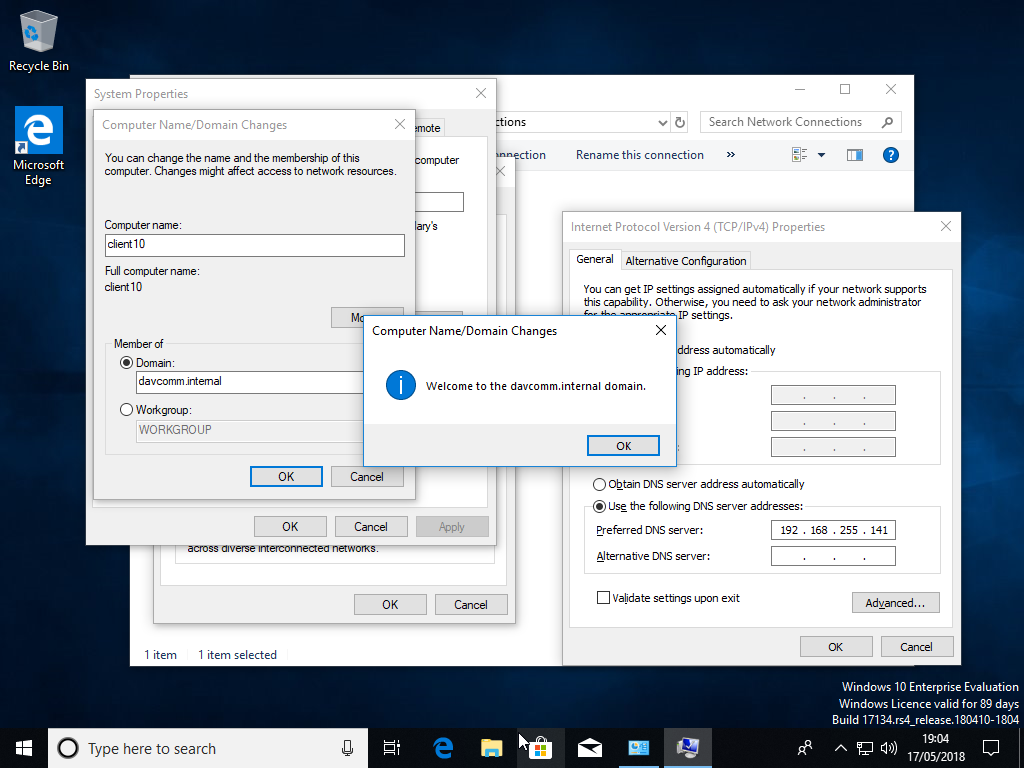
\includegraphics[width=\textwidth]{IY1D403_Windows_10_x64_Client-2018-05-17-19-04-55}
          \caption{Connecting the client to the domain}
          \label{fig:task3:win10client_04}
        \end{figure}
    \end{enumerate}
\end{enumerate}

\subsubsection{Creating user accounts within Active Directory}
\begin{enumerate}[series=task3methodology2]
  \item Open `Active Directory Users and Computers' from `Tools' in the `Server Manager' -- in `Users' we can see the accounts and security groups that are included by default.
    \begin{figure}[H]
      \centering
      \captionsetup{skip=2pt}
      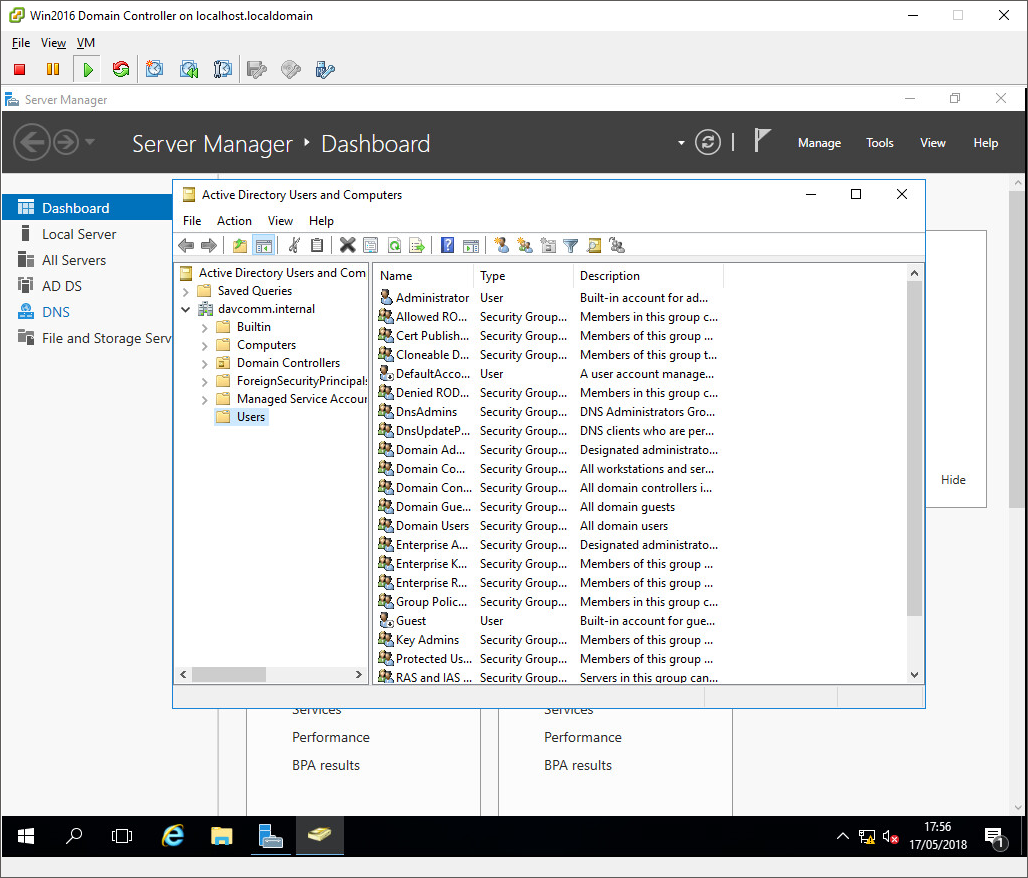
\includegraphics[width=\textwidth]{task3_01_ad_config_01}
      \caption{Active Directory Users and Computers default users}
      \label{fig:task3:ad_config_01}
    \end{figure}
  \item Create a new organisational unit called `Resources' and sub-OUs within `Resources' based on the privilege levels of users within the domain.
  \item Create an account under the `SysOps' OU for myself.
    \begin{figure}[H]
      \centering
      \captionsetup{skip=2pt}
      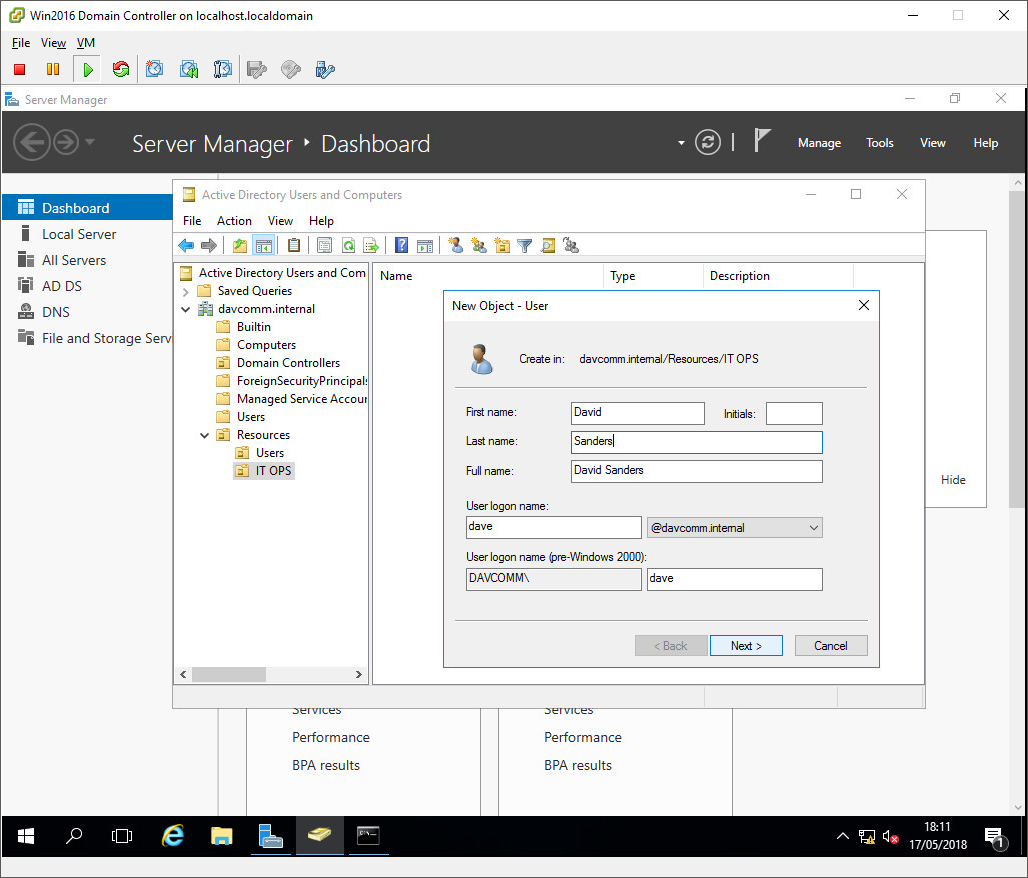
\includegraphics[width=\textwidth]{task3_01_ad_config_02}
      \caption{Setting the information for a new User in AD}
      \label{fig:task3:ad_config_02}
    \end{figure}
    \begin{figure}[H]
      \centering
      \captionsetup{skip=2pt}
      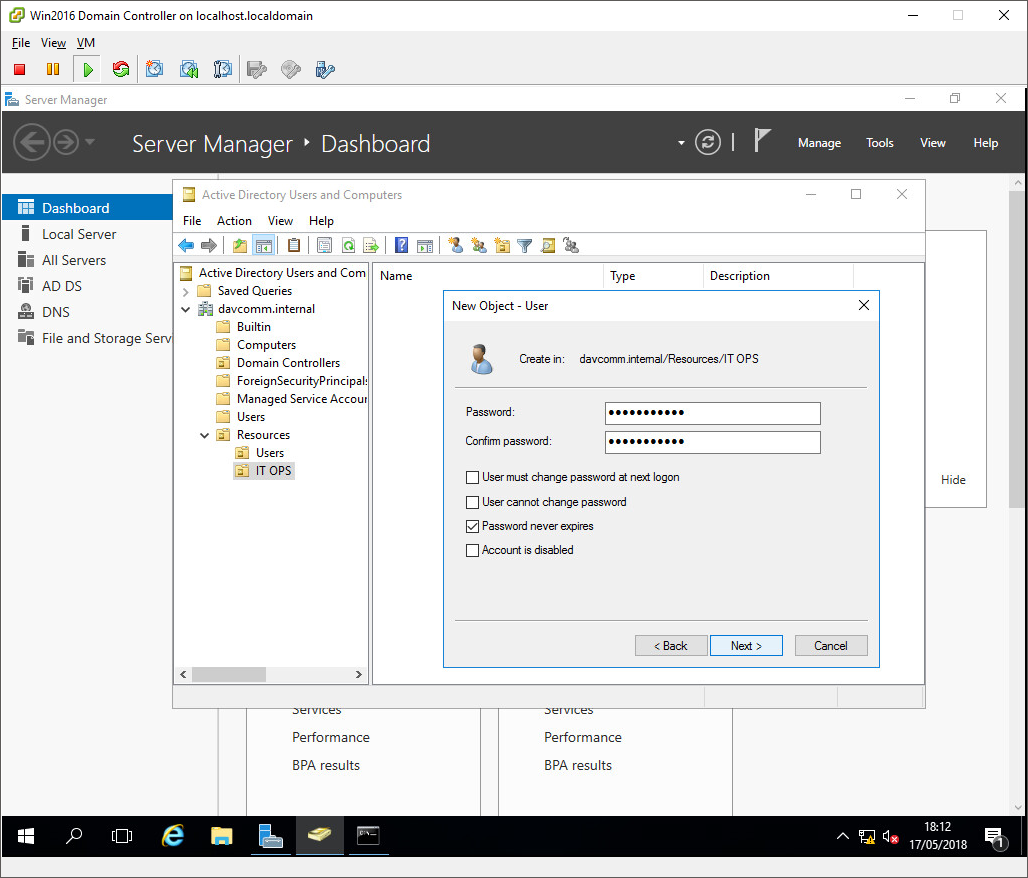
\includegraphics[width=\textwidth]{task3_01_ad_config_03}
      \caption{Setting the password for a new User in AD}
      \label{fig:task3:ad_config_03}
    \end{figure}
    \begin{figure}[H]
      \centering
      \captionsetup{skip=2pt}
      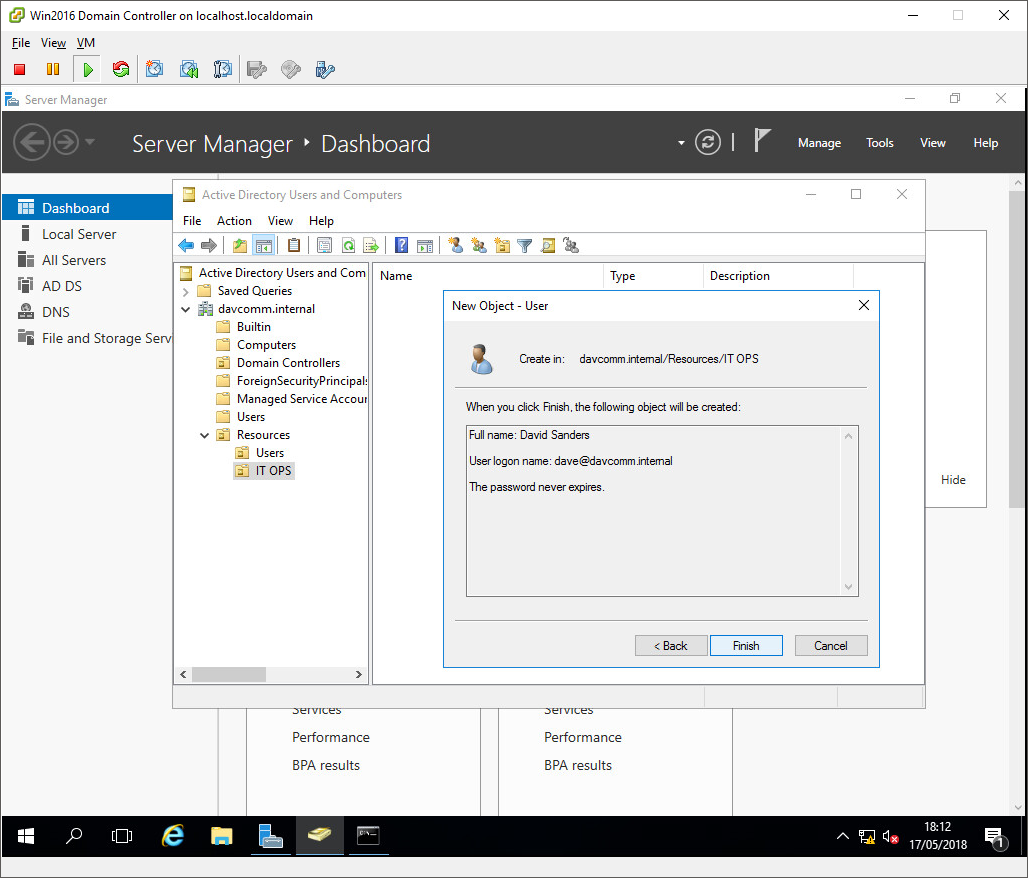
\includegraphics[width=\textwidth]{task3_01_ad_config_04}
      \caption{Reviewing and accepting the creation of a new User in AD}
      \label{fig:task3:ad_config_04}
    \end{figure}
  \item Create a second SysOp.
    \begin{figure}[H]
      \centering
      \captionsetup{skip=2pt}
      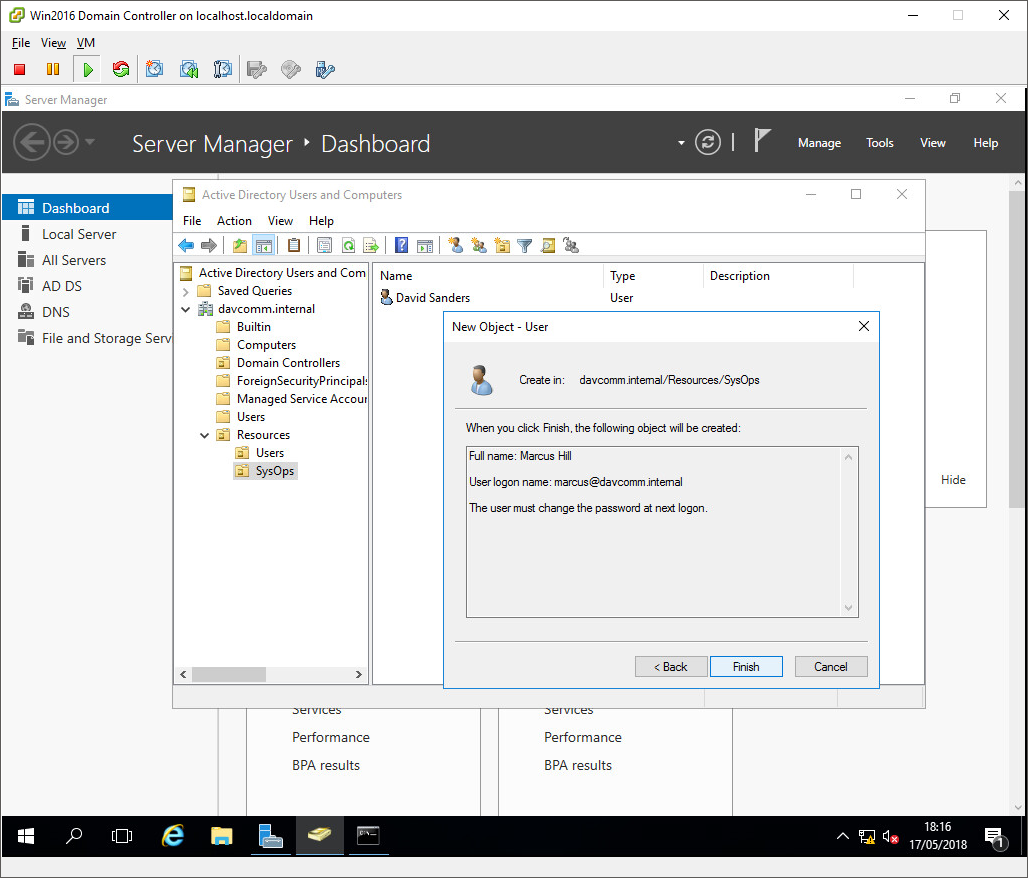
\includegraphics[width=\textwidth]{task3_01_ad_config_06_marcus}
      \caption{Creating a second User in AD under `SysOps'}
      \label{fig:task3:ad_config_06}
    \end{figure}
  \item Create three unprivileged Users in AD as shown in the screenshot below.
    \begin{figure}[H]
      \centering
      \captionsetup{skip=2pt}
      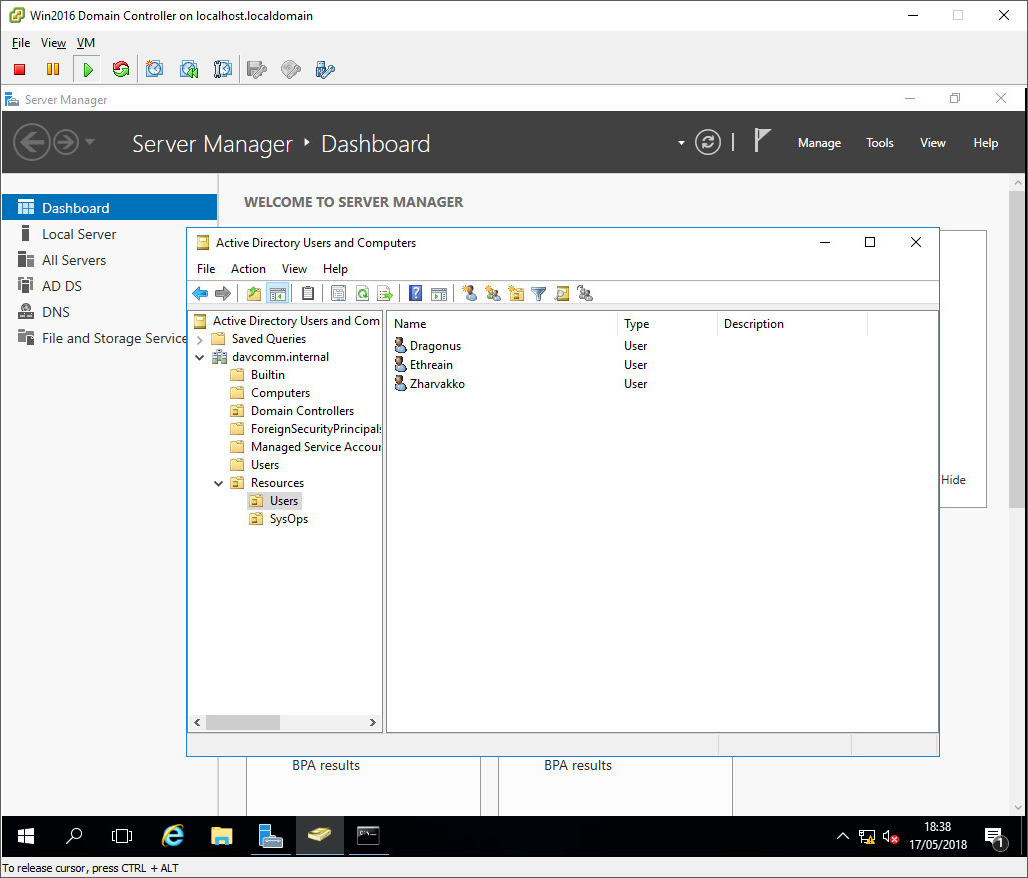
\includegraphics[width=\textwidth]{task3_01_ad_config_08}
      \caption{Active Directory > davcomm.internal > Resources > Users}
      \label{fig:task3:ad_config_08}
    \end{figure}
  \item Add the `SysOps' to the Domain Admins group to give them the privileges required for them to manage the domain.
    \begin{figure}[H]
      \centering
      \captionsetup{skip=2pt}
      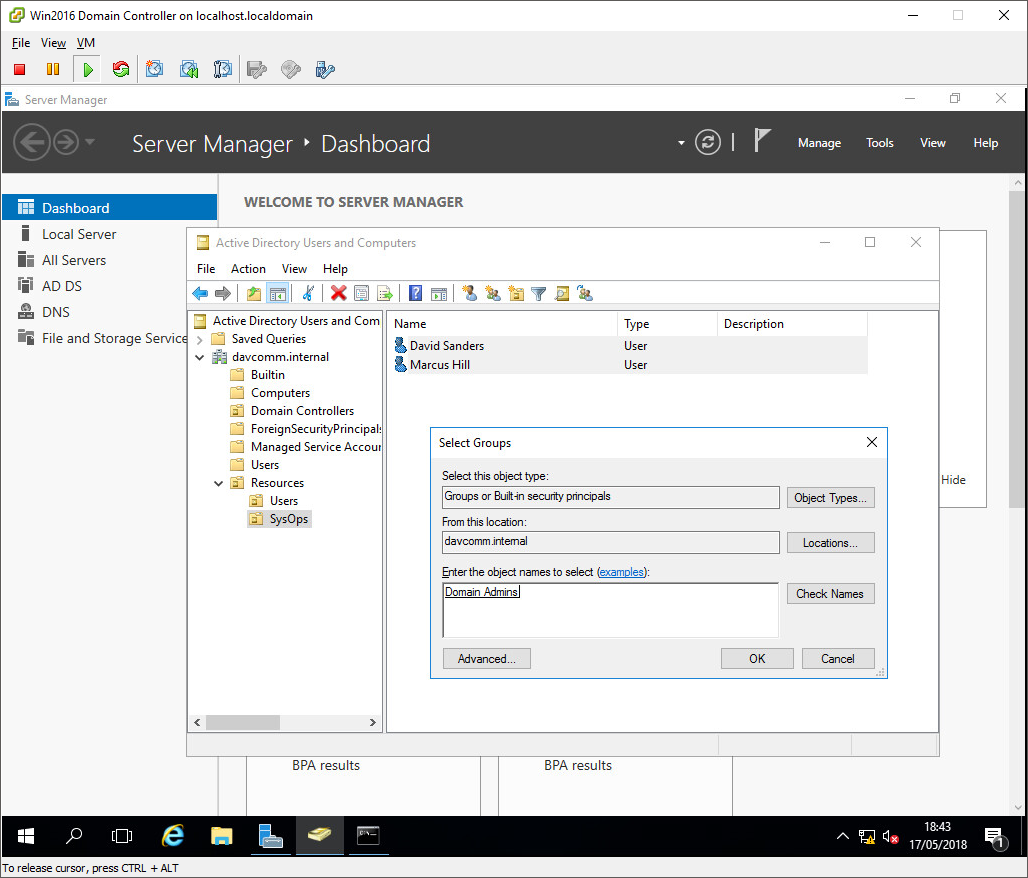
\includegraphics[width=\textwidth]{task3_01_ad_config_10}
      \caption{Adding the `SysOps' to the Domain Admins group}
      \label{fig:task3:ad_config_10}
    \end{figure}
    \begin{figure}[H]
      \centering
      \captionsetup{skip=2pt}
      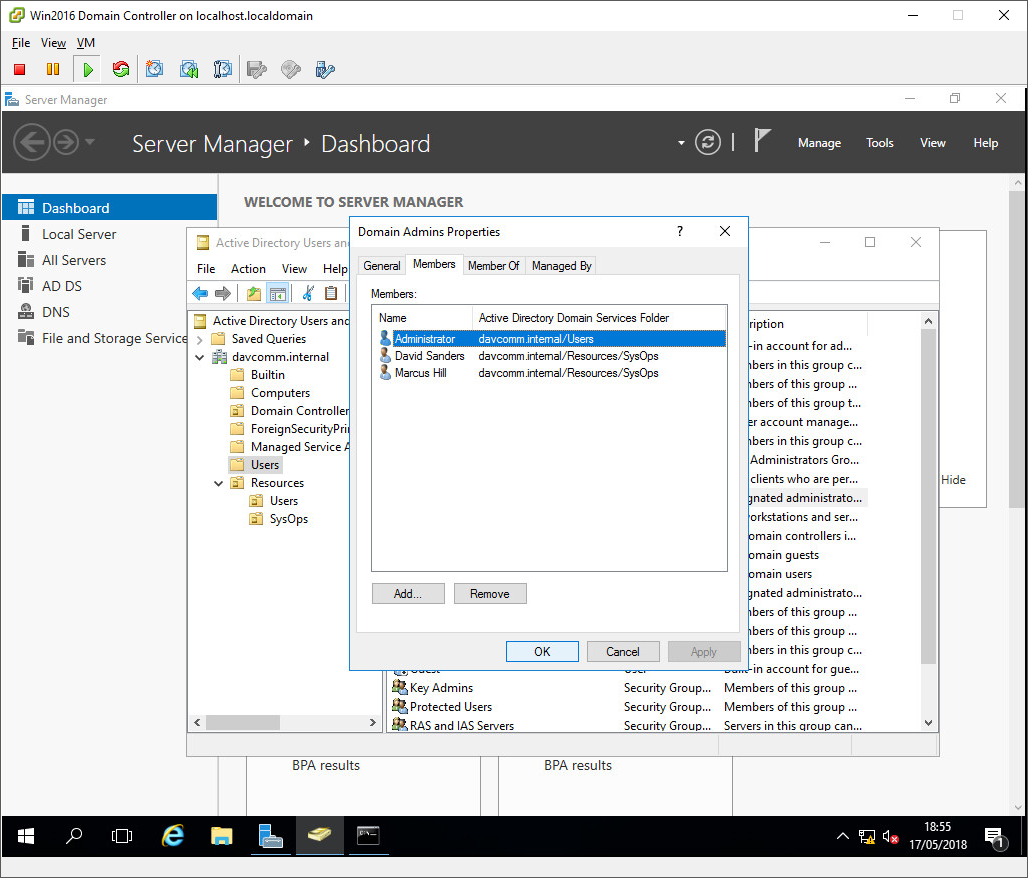
\includegraphics[width=\textwidth]{task3_01_ad_config_11}
      \caption{Reviewing the members of the Domain Admins group}
      \label{fig:task3:ad_config_11}
    \end{figure}
  \item Login to one of the user accounts on the client to prove that the Active Directory configuration has been performed successfully.
    \begin{figure}[H]
      \centering
      \captionsetup{skip=2pt}
      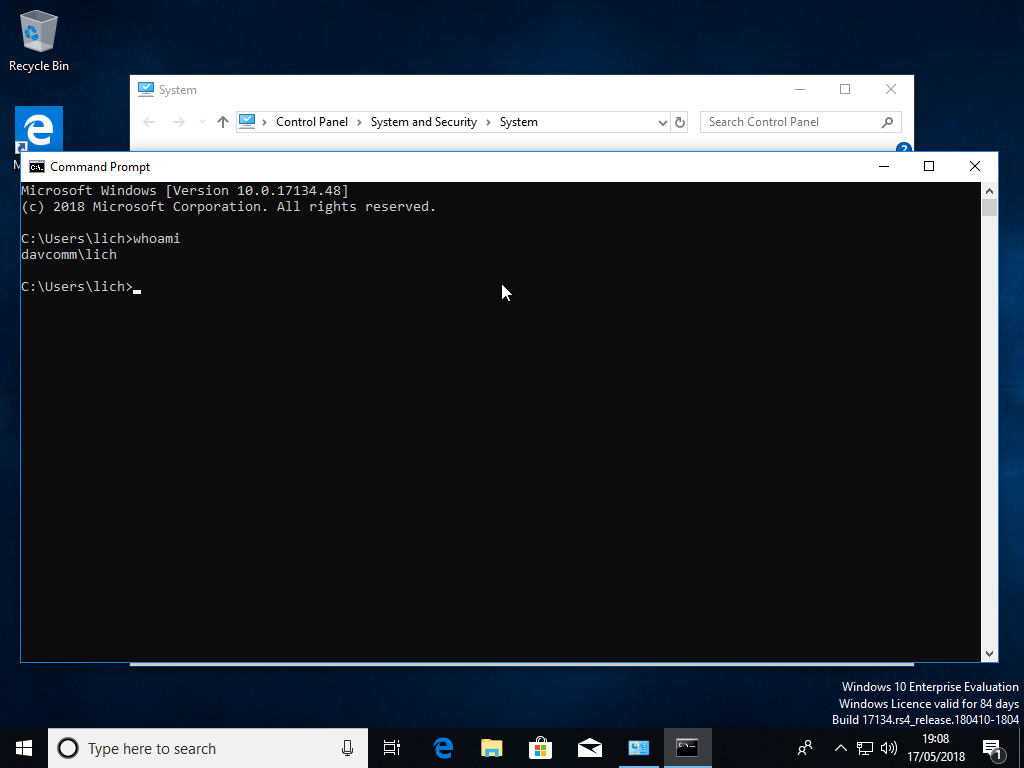
\includegraphics[width=\textwidth]{IY1D403_Windows_10_x64_Client-2018-05-17-19-08-34}
      \caption{Checking on the client that the AD configuration works properly}
      \label{fig:task3:win10client_05}
    \end{figure}
\end{enumerate}
